% ============================================================================
% QUANTUM FOOD OPTIMIZATION - BEAMER PRESENTATION
% A Beautiful Technical Presentation - Best of Both Versions
% Author: Edoardo Spigarolo
% ============================================================================

\documentclass[aspectratio=169,10pt]{beamer}

% ============================================================================
% THEME AND COLORS
% ============================================================================
\usetheme{default}
\usecolortheme{default}

% Custom colors - Professional blue-green quantum theme
\definecolor{primaryBlue}{RGB}{0, 84, 147}
\definecolor{secondaryBlue}{RGB}{0, 119, 182}
\definecolor{accentTeal}{RGB}{0, 150, 136}
\definecolor{accentGreen}{RGB}{76, 175, 80}
\definecolor{warmOrange}{RGB}{255, 152, 0}
\definecolor{alertRed}{RGB}{244, 67, 54}
\definecolor{lightBg}{RGB}{245, 248, 250}
\definecolor{darkText}{RGB}{33, 37, 41}
\definecolor{mutedGray}{RGB}{108, 117, 125}

% Set main colors
\setbeamercolor{palette primary}{bg=primaryBlue,fg=white}
\setbeamercolor{palette secondary}{bg=secondaryBlue,fg=white}
\setbeamercolor{palette tertiary}{bg=accentTeal,fg=white}
\setbeamercolor{structure}{fg=primaryBlue}
\setbeamercolor{title}{fg=white}
\setbeamercolor{frametitle}{fg=primaryBlue,bg=white}
\setbeamercolor{normal text}{fg=darkText}
\setbeamercolor{block title}{bg=primaryBlue,fg=white}
\setbeamercolor{block body}{bg=lightBg,fg=darkText}
\setbeamercolor{block title example}{bg=accentGreen,fg=white}
\setbeamercolor{block body example}{bg=lightBg,fg=darkText}
\setbeamercolor{block title alerted}{bg=alertRed,fg=white}
\setbeamercolor{block body alerted}{bg=lightBg,fg=darkText}
\setbeamercolor{itemize item}{fg=primaryBlue}
\setbeamercolor{itemize subitem}{fg=secondaryBlue}
\setbeamercolor{enumerate item}{fg=primaryBlue}

% ============================================================================
% PACKAGES
% ============================================================================
\usepackage[utf8]{inputenc}
\usepackage[T1]{fontenc}
\usepackage{lmodern}
\usepackage{amsmath,amssymb,amsfonts}
\usepackage{graphicx}
\usepackage{tikz}
\usetikzlibrary{shapes,arrows,positioning,calc,decorations.pathmorphing,backgrounds,fit,automata,shadows,patterns,arrows.meta}
\usepackage{pgfplots}
\pgfplotsset{compat=1.18}
\usepackage{booktabs}
\usepackage{multirow}
\usepackage{array}
\usepackage{xcolor}
\usepackage{fontawesome5}
\usepackage{tcolorbox}
\tcbuselibrary{skins,breakable}
\usepackage{hyperref}

% Graphics path - use actual location of plots
\graphicspath{{../plots/}}

% ============================================================================
% CUSTOM BEAMER TEMPLATE
% ============================================================================

% Remove navigation symbols
\setbeamertemplate{navigation symbols}{}

% Reduce margins for denser slides
\setbeamersize{text margin left=0.6cm,text margin right=0.6cm}

% Custom headline with gradient
\setbeamertemplate{headline}{%
    \begin{tikzpicture}[remember picture,overlay]
        \fill[primaryBlue] (current page.north west) rectangle ([yshift=-0.5cm]current page.north east);
        \fill[secondaryBlue,opacity=0.4] ([yshift=-0.25cm]current page.north west) rectangle ([yshift=-0.5cm]current page.north east);
    \end{tikzpicture}
    \vspace{0.5cm}
}

% Custom footline with page numbers and info
\setbeamertemplate{footline}{%
    \begin{tikzpicture}[remember picture,overlay]
        \fill[lightBg] (current page.south west) rectangle ([yshift=0.4cm]current page.south east);
        \draw[primaryBlue,line width=0.5pt] ([yshift=0.4cm]current page.south west) -- ([yshift=0.4cm]current page.south east);
        \node[anchor=west,text=mutedGray,font=\tiny] at ([xshift=0.5cm,yshift=0.2cm]current page.south west) {Food Production Optimization | Quantum Computing};
        \node[anchor=east,text=mutedGray,font=\tiny] at ([xshift=-0.5cm,yshift=0.2cm]current page.south east) {E. Spigarolo | \insertframenumber/\inserttotalframenumber};
    \end{tikzpicture}
    \vspace{0.4cm}
}

% Custom frame title
\setbeamertemplate{frametitle}{%
    \vspace{0.15cm}
    \begin{beamercolorbox}[wd=\paperwidth,ht=1cm,dp=0.2cm]{frametitle}
        \hspace{0.4cm}\usebeamerfont{frametitle}\insertframetitle
        \ifx\insertframesubtitle\empty\else
            \par\hspace{0.4cm}{\small\color{mutedGray}\insertframesubtitle}
        \fi
    \end{beamercolorbox}
}

% Custom itemize bullets
\setbeamertemplate{itemize item}{\footnotesize\raisebox{0.1em}{\tikz\fill[primaryBlue] (0,0) circle (0.12em);}}
\setbeamertemplate{itemize subitem}{\footnotesize\raisebox{0.1em}{\tikz\fill[secondaryBlue] (0,0) circle (0.08em);}}
\setbeamertemplate{itemize subsubitem}{\footnotesize\raisebox{0.1em}{\tikz\draw[accentTeal,thick] (0,0) circle (0.08em);}}

% ============================================================================
% CUSTOM COMMANDS AND ENVIRONMENTS
% ============================================================================

% Highlight box
\newtcolorbox{highlightbox}[1][]{
    enhanced,
    colback=lightBg,
    colframe=primaryBlue,
    boxrule=1.5pt,
    arc=4pt,
    left=6pt,right=6pt,top=5pt,bottom=5pt,
    shadow={1mm}{-1mm}{0mm}{black!20},
    #1
}

% Key insight box
\newtcolorbox{keyinsight}[1][Key Insight]{
    enhanced,
    colback=accentTeal!10,
    colframe=accentTeal,
    boxrule=1.5pt,
    arc=5pt,
    fonttitle=\bfseries\small\color{white},
    title=#1,
    coltitle=white,
    attach boxed title to top left={xshift=8pt,yshift=-\tcboxedtitleheight/2},
    boxed title style={colback=accentTeal,arc=3pt,boxrule=0pt}
}

% Result box
\newtcolorbox{resultbox}[1][Result]{
    enhanced,
    colback=accentGreen!10,
    colframe=accentGreen,
    boxrule=1.5pt,
    arc=5pt,
    fonttitle=\bfseries\small\color{white},
    title=#1,
    coltitle=white,
    attach boxed title to top left={xshift=8pt,yshift=-\tcboxedtitleheight/2},
    boxed title style={colback=accentGreen,arc=3pt,boxrule=0pt}
}

% Warning box
\newtcolorbox{warningbox}[1][Warning]{
    enhanced,
    colback=warmOrange!10,
    colframe=warmOrange,
    boxrule=1.5pt,
    arc=5pt,
    fonttitle=\bfseries\small\color{white},
    title=#1,
    coltitle=white,
    attach boxed title to top left={xshift=8pt,yshift=-\tcboxedtitleheight/2},
    boxed title style={colback=warmOrange,arc=3pt,boxrule=0pt}
}

% Metric display
\newcommand{\metricbox}[3]{%
    \begin{tikzpicture}
        \node[rounded corners=5pt, fill=#3!15, draw=#3, line width=1.5pt, 
              minimum width=2.5cm, minimum height=1.3cm, align=center,
              drop shadow={shadow xshift=0.5mm, shadow yshift=-0.5mm, opacity=0.3}] {
            {\Large\bfseries\color{#3}#1}\\[1pt]
            {\scriptsize\color{darkText}#2}
        };
    \end{tikzpicture}
}

% ============================================================================
% TITLE PAGE SETUP
% ============================================================================
\title[Food Optimization]{\textbf{Food Production Optimization}}
\subtitle{Quantum Annealing for Sustainable Agriculture\\[0.3em]{\small Phase 3 \& 4 Report}}
\author{Edoardo Spigarolo}
\institute{EPFL | Open Quantum Initiative}
\date{January 2026}

% ============================================================================
% DOCUMENT START
% ============================================================================
\begin{document}

% ============================================================================
% TITLE SLIDE
% ============================================================================
{
\setbeamertemplate{headline}{}
\setbeamertemplate{footline}{}
\begin{frame}[plain]
\begin{tikzpicture}[remember picture,overlay]
    % Background gradient
    \fill[primaryBlue] (current page.north west) rectangle (current page.south east);
    \shade[top color=primaryBlue,bottom color=secondaryBlue!80!primaryBlue] 
        ([yshift=-3cm]current page.north west) rectangle (current page.south east);
    
    % Decorative quantum circles
    \foreach \i in {1,...,12} {
        \pgfmathsetmacro{\x}{rand*16}
        \pgfmathsetmacro{\y}{rand*9}
        \pgfmathsetmacro{\r}{0.1+rand*0.3}
        \fill[white,opacity=0.08] (\x,\y) circle (\r);
    }
    
    % Decorative lines
    \draw[white,opacity=0.1,line width=0.5pt] ([xshift=2cm,yshift=-2cm]current page.north west) -- ([xshift=-2cm,yshift=2cm]current page.south east);
    \draw[white,opacity=0.1,line width=0.5pt] ([xshift=4cm,yshift=-2cm]current page.north west) -- ([xshift=-4cm,yshift=2cm]current page.south east);
    
    % Main title
    \node[white,font=\fontsize{32}{36}\selectfont\bfseries,align=center] 
        at ([yshift=1.8cm]current page.center) {Food Production Optimization};
    
    % Subtitle
    \node[white!90,font=\large,align=center] 
        at ([yshift=0.5cm]current page.center) {Quantum Annealing for Sustainable Agriculture};
    
    % Phase indicator
    \node[rounded corners=8pt,fill=accentTeal,text=white,font=\small\bfseries,
          inner sep=6pt,drop shadow={opacity=0.3}] 
        at ([yshift=-0.6cm]current page.center) {Phase 3 \& 4 Report};
    
    % Author
    \node[white,font=\normalsize] at ([yshift=-2cm]current page.center) {Edoardo Spigarolo};
    
    % Institution
    \node[white!70,font=\small] at ([yshift=-2.6cm]current page.center) 
        {EPFL \quad$\bullet$\quad Open Quantum Initiative \quad$\bullet$\quad January 2026};
    
    % Bottom decoration
    \fill[white,opacity=0.05] (current page.south west) rectangle ([yshift=0.8cm]current page.south east);
    
    % SDG icons at bottom
    \node[white!60,font=\tiny] at ([yshift=0.4cm]current page.south) 
        {\faLeaf\quad SDG 2 \quad$\bullet$\quad SDG 3 \quad$\bullet$\quad SDG 12 \quad$\bullet$\quad SDG 13 \quad\faGlobe};
\end{tikzpicture}
\end{frame}
}

% ============================================================================
% OUTLINE
% ============================================================================
\begin{frame}{Outline}
    \begin{columns}[T]
        \begin{column}{0.48\textwidth}
            % Left column with visual outline
            \begin{tikzpicture}[
                every node/.style={font=\small},
                section/.style={rounded corners=3pt,fill=primaryBlue!10,draw=primaryBlue,
                               minimum width=5.5cm,minimum height=0.7cm,align=left,
                               text=darkText,font=\small\bfseries},
                item/.style={text=mutedGray,font=\scriptsize,align=left}
            ]
                % Part I
                \node[section] (p1) at (0,0) {\color{primaryBlue}\faBook\ Part I: Background \& Setup};
                \node[item,below=0.1cm of p1.south west,anchor=north west,xshift=0.3cm] {
                    1. Problem \& Motivation\\
                    2. Mathematical Formulation\\
                    3. Quantum Hardware\\
                    4. Decomposition Strategies
                };
                
                % Part II
                \node[section,below=1.8cm of p1] (p2) {\color{accentTeal}\faFlask\ Part II: Experimental Studies};
                \node[item,below=0.1cm of p2.south west,anchor=north west,xshift=0.3cm] {
                    5. Study 1: Hybrid Solver\\
                    6. Study 2: Pure QPU\\
                    7. Study 3: Quantum Improvement
                };
            \end{tikzpicture}
        \end{column}
        \begin{column}{0.48\textwidth}
            \begin{tikzpicture}[
                every node/.style={font=\small},
                section/.style={rounded corners=3pt,fill=primaryBlue!10,draw=primaryBlue,
                               minimum width=5.5cm,minimum height=0.7cm,align=left,
                               text=darkText,font=\small\bfseries},
                item/.style={text=mutedGray,font=\scriptsize,align=left}
            ]
                % Part III
                \node[section] (p3) at (0,0) {\color{accentGreen}\faChartBar\ Part III: Analysis};
                \node[item,below=0.1cm of p3.south west,anchor=north west,xshift=0.3cm] {
                    8. Results Comparison\\
                    9. Solution Quality\\
                    10. Hardware Effects \& Noise\\
                    11. Grid Refinement
                };
                
                % Part IV
                \node[section,below=1.8cm of p3] (p4) {\color{warmOrange}\faLightbulb\ Part IV: Conclusions};
                \node[item,below=0.1cm of p4.south west,anchor=north west,xshift=0.3cm] {
                    12. Key Takeaways\\
                    13. Impact Assessment\\
                    14. Future Directions
                };
            \end{tikzpicture}
        \end{column}
    \end{columns}
    
    \vspace{0.4cm}
    \centering
    
\begin{tikzpicture}
        \node[rounded corners=3pt,fill=primaryBlue!5,draw=primaryBlue!30,
              font=\scriptsize,text=mutedGray,inner sep=4pt] {
            \faClockFour\ \textbf{40 minutes} \quad$\bullet$\quad 
            \faSlideshare\ \textbf{42 slides} \quad$\bullet$\quad 
            \faChartLine\ \textbf{3 studies}
        };
    \end{tikzpicture}
\end{frame}

% ============================================================================
% SECTION 1: PROBLEM & MOTIVATION
% ============================================================================
\section{Problem \& Motivation}

\begin{frame}{The Challenge: Sustainable Food Production}
    \framesubtitle{Optimizing crop allocation across multiple objectives}
    
    \begin{columns}[T]
        \begin{column}{0.55\textwidth}
            % Visual problem representation
            \begin{tikzpicture}[scale=0.85,transform shape]
                % Central node
                \node[circle,fill=primaryBlue,text=white,minimum size=1.8cm,font=\small\bfseries,
                      drop shadow={opacity=0.3}] (center) at (0,0) {Optimize};
                
                % Surrounding objectives
                \foreach \angle/\color/\icon/\text in {
                    90/accentGreen/\faCarrot/Nutrition,
                    162/secondaryBlue/\faLeaf/Environment,
                    234/warmOrange/\faDollarSign/Affordability,
                    306/accentTeal/\faRecycle/Sustainability,
                    18/alertRed/\faBalanceScale/Diversity
                } {
                    \node[circle,fill=\color!20,draw=\color,minimum size=1.2cm,
                          font=\tiny,align=center,line width=1pt] 
                        at (\angle:2.2cm) {\icon\\\text};
                    \draw[->,\color,thick] (center) -- (\angle:1.5cm);
                }
            \end{tikzpicture}
            
            \vspace{0.3cm}
            \small\textbf{Problem Complexity:}
            \begin{itemize}\scriptsize
                \item 27 crops across 5 food groups
                \item Multiple farms with varying sizes
                \item Min/max diversity constraints
                \item Rotation synergies (Variant B)
            \end{itemize}
        \end{column}
        \begin{column}{0.43\textwidth}
            \textbf{Relevant SDGs:}
            \vspace{0.2cm}
            
            \begin{tikzpicture}[
                sdg/.style={rounded corners=3pt,minimum width=4.5cm,minimum height=0.55cm,
                           font=\scriptsize,align=left,text=white,drop shadow={opacity=0.2}}
            ]
                \node[sdg,fill=warmOrange] at (0,0) {\faSeedling\ SDG 2: Zero Hunger};
                \node[sdg,fill=accentGreen] at (0,-0.75) {\faHeartbeat\ SDG 3: Good Health};
                \node[sdg,fill=accentTeal] at (0,-1.5) {\faRecycle\ SDG 12: Responsible Consumption};
                \node[sdg,fill=secondaryBlue] at (0,-2.25) {\faCloudSun\ SDG 13: Climate Action};
            \end{tikzpicture}
            
            \vspace{0.3cm}
            \begin{keyinsight}[Why Quantum?]
                \scriptsize Classical solvers struggle with frustrated constraints. Quantum annealing naturally explores rugged energy landscapes.
            \end{keyinsight}
        \end{column}
    \end{columns}
\end{frame}

\begin{frame}{Data: Real-World Agricultural Dataset}
    \framesubtitle{27 crops from Bangladesh \& Indonesia (GAIN)}
    
    \begin{columns}[T]
        \begin{column}{0.48\textwidth}
            \small\textbf{Crop Database:}
            \vspace{0.1cm}
            
            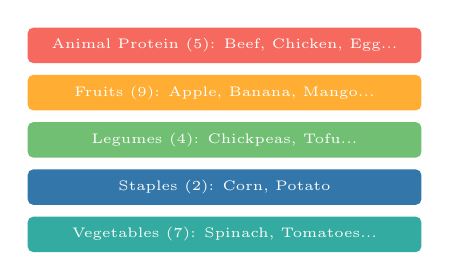
\begin{tikzpicture}[
                group/.style={rounded corners=2pt,minimum width=5cm,minimum height=0.45cm,
                             font=\tiny,align=left,text=white}
            ]
                \node[group,fill=alertRed!80] at (0,0) {Animal Protein (5): Beef, Chicken, Egg...};
                \node[group,fill=warmOrange!80] at (0,-0.6) {Fruits (9): Apple, Banana, Mango...};
                \node[group,fill=accentGreen!80] at (0,-1.2) {Legumes (4): Chickpeas, Tofu...};
                \node[group,fill=primaryBlue!80] at (0,-1.8) {Staples (2): Corn, Potato};
                \node[group,fill=accentTeal!80] at (0,-2.4) {Vegetables (7): Spinach, Tomatoes...};
            \end{tikzpicture}
            
            \vspace{0.3cm}
            \begin{highlightbox}
                \centering\small\textbf{Total: 27 crops}\\
                \scriptsize across 5 food groups
            \end{highlightbox}
        \end{column}
        \begin{column}{0.48\textwidth}
            \small\textbf{Benefit Score Calculation:}
            \begin{equation*}
                B_c = \sum_i w_i \cdot v_{i,c}
            \end{equation*}
            
            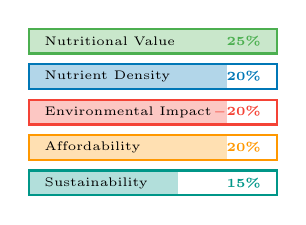
\begin{tikzpicture}[scale=0.9,transform shape]
                % Nutritional Value - 25%
                \fill[accentGreen!30] (0,0) rectangle (3.5,0.35);
                \draw[accentGreen,thick] (0,0) rectangle (3.5,0.35);
                \node[font=\tiny,anchor=west] at (0.1,0.175) {Nutritional Value};
                \node[font=\tiny\bfseries,anchor=east,accentGreen] at (3.4,0.175) {25\%};
                % Nutrient Density - 20%
                \fill[secondaryBlue!30] (0,-0.5) rectangle (2.8,-0.15);
                \draw[secondaryBlue,thick] (0,-0.5) rectangle (3.5,-0.15);
                \node[font=\tiny,anchor=west] at (0.1,-0.325) {Nutrient Density};
                \node[font=\tiny\bfseries,anchor=east,secondaryBlue] at (3.4,-0.325) {20\%};
                % Environmental Impact - 20%
                \fill[alertRed!30] (0,-1.0) rectangle (2.8,-0.65);
                \draw[alertRed,thick] (0,-1.0) rectangle (3.5,-0.65);
                \node[font=\tiny,anchor=west] at (0.1,-0.825) {Environmental Impact};
                \node[font=\tiny\bfseries,anchor=east,alertRed] at (3.4,-0.825) {$-$20\%};
                % Affordability - 20%
                \fill[warmOrange!30] (0,-1.5) rectangle (2.8,-1.15);
                \draw[warmOrange,thick] (0,-1.5) rectangle (3.5,-1.15);
                \node[font=\tiny,anchor=west] at (0.1,-1.325) {Affordability};
                \node[font=\tiny\bfseries,anchor=east,warmOrange] at (3.4,-1.325) {20\%};
                % Sustainability - 15%
                \fill[accentTeal!30] (0,-2.0) rectangle (2.1,-1.65);
                \draw[accentTeal,thick] (0,-2.0) rectangle (3.5,-1.65);
                \node[font=\tiny,anchor=west] at (0.1,-1.825) {Sustainability};
                \node[font=\tiny\bfseries,anchor=east,accentTeal] at (3.4,-1.825) {15\%};
            \end{tikzpicture}
            
            \vspace{0.2cm}
            \begin{warningbox}[Note]
                \scriptsize Environmental impact is \textbf{negatively weighted} to penalize high-impact crops.
            \end{warningbox}
        \end{column}
    \end{columns}
\end{frame}

\begin{frame}{Benefit Score Distribution}
    \centering
    \includegraphics[width=0.85\textwidth]{02_benefit_heatmap.png}
    
    \vspace{0.2cm}
    \small Heatmap of benefit scores (5 components) across 27 crops.
\end{frame}

% ============================================================================
% SECTION 2: MATHEMATICAL FORMULATION
% ============================================================================
\section{Mathematical Formulation}

\begin{frame}{Problem Variant A: Binary Crop Allocation}
    \framesubtitle{Constrained Quadratic Model (CQM)}
    
    \begin{columns}[T]
        \begin{column}{0.48\textwidth}
            \textbf{Decision Variables:}
            \begin{itemize}\small
                \item $Y_{f,c} \in \{0,1\}$: crop $c$ on farm $f$
                \item $U_c \in \{0,1\}$: crop $c$ used anywhere
            \end{itemize}
            
            \vspace{0.2cm}
            \textbf{Objective:} Maximize benefit
            \begin{equation*}
                \max Z = \frac{1}{A_{\text{total}}} \sum_{f,c} L_f \cdot B_c \cdot Y_{f,c}
            \end{equation*}
            
            \vspace{0.2cm}
            \begin{highlightbox}
                \centering\small
                \textbf{Problem Size at 1,000 farms:}\\
                \Large\textcolor{primaryBlue}{27,027} \small variables
            \end{highlightbox}
        \end{column}
        \begin{column}{0.48\textwidth}
            \textbf{Constraints:}
            
            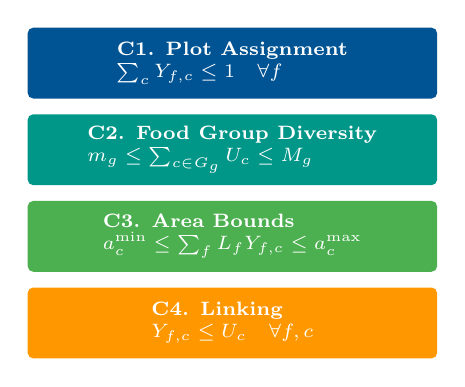
\begin{tikzpicture}[
                constraint/.style={rounded corners=2pt,minimum width=5.2cm,
                                  minimum height=0.9cm,font=\scriptsize,align=left,
                                  text=white,inner sep=4pt}
            ]
                \node[constraint,fill=primaryBlue] at (0,0) {
                    \textbf{C1. Plot Assignment}\\
                    $\sum_{c} Y_{f,c} \leq 1 \quad \forall f$
                };
                \node[constraint,fill=accentTeal] at (0,-1.1) {
                    \textbf{C2. Food Group Diversity}\\
                    $m_g \leq \sum_{c \in G_g} U_c \leq M_g$
                };
                \node[constraint,fill=accentGreen] at (0,-2.2) {
                    \textbf{C3. Area Bounds}\\
                    $a^{\min}_c \leq \sum_f L_f Y_{f,c} \leq a^{\max}_c$
                };
                \node[constraint,fill=warmOrange] at (0,-3.3) {
                    \textbf{C4. Linking}\\
                    $Y_{f,c} \leq U_c \quad \forall f,c$
                };
            \end{tikzpicture}
        \end{column}
    \end{columns}
\end{frame}

\begin{frame}{Problem Variant B: Multi-Period Rotation}
    \framesubtitle{Enhanced formulation with frustrated constraints}
    
    \begin{columns}[T]
        \begin{column}{0.55\textwidth}
            \small\textbf{Enhanced Formulation:}
            \begin{itemize}\scriptsize
                \item 6 aggregated crop families (not 27)
                \item 3-period temporal horizon ($T=3$)
                \item Quadratic rotation synergies
                \item Frustrated spatial interactions
            \end{itemize}
            
            \vspace{0.2cm}
            \textbf{Rotation Objective:}
            \begin{equation*}
                Z_{\text{rot}} = \sum_{f,t} \sum_{c,c'} S_{c,c'} \cdot x_{f,c,t} \cdot x_{f,c',t+1}
            \end{equation*}
            
            \textbf{Combined:}
            \begin{equation*}
                \max Z = (1-\gamma) Z_{\text{base}} + \gamma Z_{\text{rot}}
            \end{equation*}
            
            \vspace{0.1cm}
            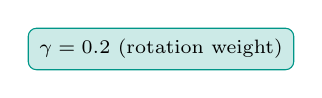
\begin{tikzpicture}
                \node[rounded corners=3pt,fill=accentTeal!20,draw=accentTeal,
                      font=\scriptsize,inner sep=4pt] {
                    $\gamma = 0.2$ (rotation weight)
                };
            \end{tikzpicture}
        \end{column}
        \begin{column}{0.43\textwidth}
            % Frustration visualization
            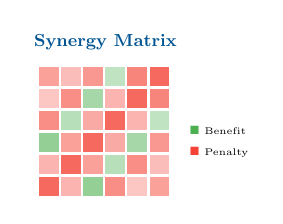
\begin{tikzpicture}[scale=0.7,transform shape]
                \node[font=\small\bfseries,primaryBlue] at (1.2,2.8) {Synergy Matrix};
                
                % Mini heatmap representation - simplified
                % Row 0
                \fill[alertRed!80] (0,0) rectangle (0.35,0.35);
                \fill[alertRed!40] (0.4,0) rectangle (0.75,0.35);
                \fill[accentGreen!60] (0.8,0) rectangle (1.15,0.35);
                \fill[alertRed!60] (1.2,0) rectangle (1.55,0.35);
                \fill[alertRed!30] (1.6,0) rectangle (1.95,0.35);
                \fill[alertRed!50] (2.0,0) rectangle (2.35,0.35);
                % Row 1
                \fill[alertRed!40] (0,0.4) rectangle (0.35,0.75);
                \fill[alertRed!80] (0.4,0.4) rectangle (0.75,0.75);
                \fill[alertRed!50] (0.8,0.4) rectangle (1.15,0.75);
                \fill[accentGreen!40] (1.2,0.4) rectangle (1.55,0.75);
                \fill[alertRed!60] (1.6,0.4) rectangle (1.95,0.75);
                \fill[alertRed!35] (2.0,0.4) rectangle (2.35,0.75);
                % Row 2
                \fill[accentGreen!60] (0,0.8) rectangle (0.35,1.15);
                \fill[alertRed!50] (0.4,0.8) rectangle (0.75,1.15);
                \fill[alertRed!80] (0.8,0.8) rectangle (1.15,1.15);
                \fill[alertRed!45] (1.2,0.8) rectangle (1.55,1.15);
                \fill[accentGreen!50] (1.6,0.8) rectangle (1.95,1.15);
                \fill[alertRed!55] (2.0,0.8) rectangle (2.35,1.15);
                % Row 3
                \fill[alertRed!60] (0,1.2) rectangle (0.35,1.55);
                \fill[accentGreen!40] (0.4,1.2) rectangle (0.75,1.55);
                \fill[alertRed!45] (0.8,1.2) rectangle (1.15,1.55);
                \fill[alertRed!80] (1.2,1.2) rectangle (1.55,1.55);
                \fill[alertRed!40] (1.6,1.2) rectangle (1.95,1.55);
                \fill[accentGreen!35] (2.0,1.2) rectangle (2.35,1.55);
                % Row 4
                \fill[alertRed!30] (0,1.6) rectangle (0.35,1.95);
                \fill[alertRed!60] (0.4,1.6) rectangle (0.75,1.95);
                \fill[accentGreen!50] (0.8,1.6) rectangle (1.15,1.95);
                \fill[alertRed!40] (1.2,1.6) rectangle (1.55,1.95);
                \fill[alertRed!80] (1.6,1.6) rectangle (1.95,1.95);
                \fill[alertRed!65] (2.0,1.6) rectangle (2.35,1.95);
                % Row 5
                \fill[alertRed!50] (0,2.0) rectangle (0.35,2.35);
                \fill[alertRed!35] (0.4,2.0) rectangle (0.75,2.35);
                \fill[alertRed!55] (0.8,2.0) rectangle (1.15,2.35);
                \fill[accentGreen!35] (1.2,2.0) rectangle (1.55,2.35);
                \fill[alertRed!65] (1.6,2.0) rectangle (1.95,2.35);
                \fill[alertRed!80] (2.0,2.0) rectangle (2.35,2.35);
                
                \node[font=\tiny,anchor=west] at (2.6,1.2) {\textcolor{accentGreen}{$\blacksquare$} Benefit};
                \node[font=\tiny,anchor=west] at (2.6,0.8) {\textcolor{alertRed}{$\blacksquare$} Penalty};
            \end{tikzpicture}
            
            \vspace{0.2cm}
            \begin{warningbox}[Frustration]
                \scriptsize \textbf{70--88\%} of rotation pairs have \textbf{negative} synergy\\[2pt]
                $\Rightarrow$ Rugged energy landscape\\
                $\Rightarrow$ Classical B\&B struggles
            \end{warningbox}
        \end{column}
    \end{columns}
\end{frame}

\begin{frame}{Rotation Parameters: Agronomic Grounding}
    \framesubtitle{Calibrated from field-trial meta-analyses}
    
    \begin{columns}[T]
        \begin{column}{0.55\textwidth}
            \begin{table}[h]\small
                \centering
                \begin{tabular}{lcc}
                    \toprule
                    \textbf{Parameter} & \textbf{Our Value} & \textbf{Literature} \\
                    \midrule
                    \rowcolor{primaryBlue!10} Rotation weight $\gamma$ & 0.2 & 0.1--0.3 \\
                    Monoculture penalty & 24\% & 15--30\% \\
                    \rowcolor{primaryBlue!10} Legume benefit & 16--25\% & 16--23\% \\
                    Spatial dampening & 0.15 & 0.1--0.2 \\
                    \rowcolor{primaryBlue!10} Frustration ratio & 70--88\% & 50--80\% \\
                    Planning horizon $T$ & 3 years & 2--5 years \\
                    \bottomrule
                \end{tabular}
            \end{table}
            
            \vspace{0.1cm}
            \begin{keyinsight}[Literature Source]
                \scriptsize Based on 3,663 paired field-trial observations across six continents (Mudare et al., 2025).
            \end{keyinsight}
        \end{column}
        \begin{column}{0.43\textwidth}
            \small\textbf{Synergy Matrix $S_{c,c'}$:}
            \begin{itemize}\scriptsize
                \item Diagonal: Monoculture penalty ($-0.24$)
                \item Legume$\to$Non-legume: Benefit ($+0.16$ to $+0.25$)
                \item Most pairs: Negative or zero
            \end{itemize}
            
            \vspace{0.3cm}
            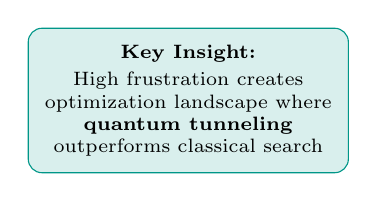
\begin{tikzpicture}
                \node[rounded corners=5pt,fill=accentTeal!15,draw=accentTeal,
                      inner sep=6pt,font=\scriptsize,align=center] {
                    \textbf{Key Insight:}\\[2pt]
                    High frustration creates\\
                    optimization landscape where\\
                    \textbf{quantum tunneling}\\
                    outperforms classical search
                };
            \end{tikzpicture}
        \end{column}
    \end{columns}
\end{frame}

% ============================================================================
% SECTION 3: QUANTUM HARDWARE
% ============================================================================
\section{Quantum Hardware \& Methods}

\begin{frame}{D-Wave Advantage: Quantum Annealing Platform}
    \framesubtitle{5,760 qubits with Pegasus topology}
    
    \begin{columns}[T]
        \begin{column}{0.45\textwidth}
            % Hardware specs as visual cards
            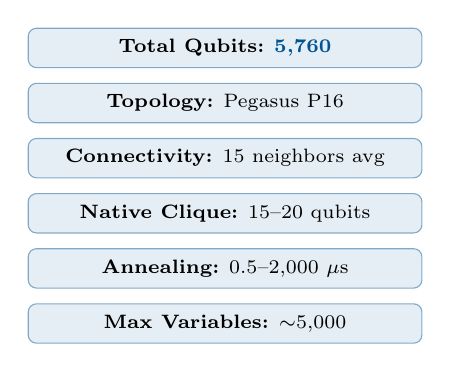
\begin{tikzpicture}[
                spec/.style={rounded corners=3pt,fill=primaryBlue!10,draw=primaryBlue!50,
                            minimum width=5cm,minimum height=0.5cm,font=\scriptsize,
                            inner sep=3pt}
            ]
                \node[spec] at (0,0) {\textbf{Total Qubits:} \textcolor{primaryBlue}{\textbf{5,760}}};
                \node[spec] at (0,-0.7) {\textbf{Topology:} Pegasus P16};
                \node[spec] at (0,-1.4) {\textbf{Connectivity:} 15 neighbors avg};
                \node[spec] at (0,-2.1) {\textbf{Native Clique:} 15--20 qubits};
                \node[spec] at (0,-2.8) {\textbf{Annealing:} 0.5--2,000 $\mu$s};
                \node[spec] at (0,-3.5) {\textbf{Max Variables:} $\sim$5,000};
            \end{tikzpicture}
        \end{column}
        \begin{column}{0.52\textwidth}
            % Pegasus topology visualization
            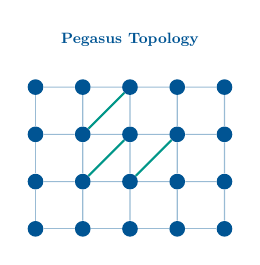
\begin{tikzpicture}[scale=0.6,transform shape]
                \node[font=\small\bfseries,primaryBlue] at (2,4) {Pegasus Topology};
                
                % Simplified topology representation
                \foreach \x in {0,...,4} {
                    \foreach \y in {0,...,3} {
                        \node[circle,fill=primaryBlue,minimum size=3pt] (n\x\y) at (\x,\y) {};
                    }
                }
                % Some connections
                \foreach \x in {0,...,3} {
                    \foreach \y in {0,...,3} {
                        \pgfmathtruncatemacro{\nx}{\x+1}
                        \draw[primaryBlue!40,thin] (n\x\y) -- (n\nx\y);
                    }
                }
                \foreach \x in {0,...,4} {
                    \foreach \y in {0,...,2} {
                        \pgfmathtruncatemacro{\ny}{\y+1}
                        \draw[primaryBlue!40,thin] (n\x\y) -- (n\x\ny);
                    }
                }
                % Cross connections
                \draw[accentTeal,thick] (n11) -- (n22);
                \draw[accentTeal,thick] (n21) -- (n32);
                \draw[accentTeal,thick] (n12) -- (n23);
            \end{tikzpicture}
            
            \vspace{0.2cm}
            \begin{resultbox}[QPU Advantage]
                \scriptsize Native cliques enable 27-crop farm subproblems with \textbf{minimal chain breaking} ($<$2\%)
            \end{resultbox}
        \end{column}
    \end{columns}
    
    \vspace{0.2cm}
    \begin{keyinsight}[Classical Baseline]
        \small Gurobi 12.0.1 with 300-second timeout, MIP gap tolerance 0.01\%
    \end{keyinsight}
\end{frame}

\begin{frame}{Decomposition Strategies for Large Problems}
    \framesubtitle{8 methods to partition problems for QPU}
    
    \begin{columns}[T]
        \begin{column}{0.48\textwidth}
            \small\textbf{Basic Methods:}
            
            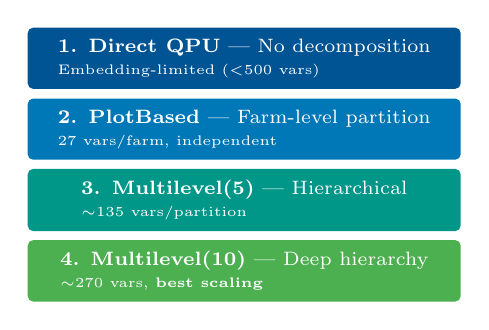
\begin{tikzpicture}[
                method/.style={rounded corners=2pt,minimum width=5.5cm,minimum height=0.7cm,
                              font=\scriptsize,align=left,inner sep=4pt,text=white}
            ]
                \node[method,fill=primaryBlue] at (0,0) {
                    \textbf{1. Direct QPU} --- No decomposition\\
                    \tiny Embedding-limited ($<$500 vars)
                };
                \node[method,fill=secondaryBlue] at (0,-0.9) {
                    \textbf{2. PlotBased} --- Farm-level partition\\
                    \tiny 27 vars/farm, independent
                };
                \node[method,fill=accentTeal] at (0,-1.8) {
                    \textbf{3. Multilevel(5)} --- Hierarchical\\
                    \tiny $\sim$135 vars/partition
                };
                \node[method,fill=accentGreen] at (0,-2.7) {
                    \textbf{4. Multilevel(10)} --- Deep hierarchy\\
                    \tiny $\sim$270 vars, \textbf{best scaling}
                };
            \end{tikzpicture}
        \end{column}
        \begin{column}{0.48\textwidth}
            \small\textbf{Advanced Methods:}
            
            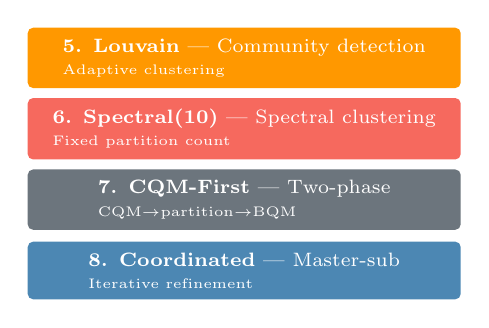
\begin{tikzpicture}[
                method/.style={rounded corners=2pt,minimum width=5.5cm,minimum height=0.7cm,
                              font=\scriptsize,align=left,inner sep=4pt,text=white}
            ]
                \node[method,fill=warmOrange] at (0,0) {
                    \textbf{5. Louvain} --- Community detection\\
                    \tiny Adaptive clustering
                };
                \node[method,fill=alertRed!80] at (0,-0.9) {
                    \textbf{6. Spectral(10)} --- Spectral clustering\\
                    \tiny Fixed partition count
                };
                \node[method,fill=mutedGray] at (0,-1.8) {
                    \textbf{7. CQM-First} --- Two-phase\\
                    \tiny CQM$\to$partition$\to$BQM
                };
                \node[method,fill=primaryBlue!70] at (0,-2.7) {
                    \textbf{8. Coordinated} --- Master-sub\\
                    \tiny Iterative refinement
                };
            \end{tikzpicture}
        \end{column}
    \end{columns}
    
    \vspace{0.3cm}
    \begin{highlightbox}
        \centering\small
        \textbf{Why Decomposition?} Full problem = 27,027 variables. QPU capacity $\approx$ 5,000. Must partition intelligently.
    \end{highlightbox}
\end{frame}

% ============================================================================
% SECTION 4: EXPERIMENTAL STUDIES
% ============================================================================
\section{Experimental Studies}

\begin{frame}{Three Complementary Studies}
    \framesubtitle{Comprehensive evaluation of quantum vs. classical performance}
    
    \centering
    \begin{tikzpicture}[
        study/.style={rounded corners=8pt,minimum width=4.2cm,minimum height=2.5cm,
                     font=\scriptsize,align=center,text=white,
                     drop shadow={opacity=0.3,shadow xshift=1mm,shadow yshift=-1mm}}
    ]
        % Study 1
        \node[study,fill=primaryBlue] (s1) at (0,0) {
            \Large\faServer\\[4pt]
            \normalsize\textbf{Study 1}\\[2pt]
            \small Hybrid Solver\\
            Benchmarking\\[4pt]
            \tiny Variant A\\
            10--1,000 farms
        };
        
        % Study 2
        \node[study,fill=accentTeal] (s2) at (5,0) {
            \Large\faMicrochip\\[4pt]
            \normalsize\textbf{Study 2}\\[2pt]
            \small Pure QPU\\
            Decomposition\\[4pt]
            \tiny 8 methods\\
            Scaling analysis
        };
        
        % Study 3
        \node[study,fill=accentGreen] (s3) at (10,0) {
            \Large\faRocket\\[4pt]
            \normalsize\textbf{Study 3}\\[2pt]
            \small Quantum\\
            Improvement\\[4pt]
            \tiny Variant B\\
            13 scenarios
        };
        
        % Arrows
        \draw[->,very thick,primaryBlue!60] (s1.east) -- node[above,font=\tiny,text=mutedGray] {inform} (s2.west);
        \draw[->,very thick,accentTeal!60] (s2.east) -- node[above,font=\tiny,text=mutedGray] {enable} (s3.west);
    \end{tikzpicture}
    
    \vspace{0.5cm}
    \begin{tikzpicture}
        \node[rounded corners=5pt,fill=lightBg,draw=mutedGray,
              font=\scriptsize,inner sep=6pt] {
            \faCheckCircle\ Establish baseline $\rightarrow$ 
            \faCheckCircle\ Analyze scaling $\rightarrow$ 
            \faCheckCircle\ Demonstrate improvement
        };
    \end{tikzpicture}
\end{frame}

\begin{frame}{Study 1: Hybrid Solver Results}
    \framesubtitle{D-Wave CQM vs Gurobi on Variant A}
    
    \centering
    \includegraphics[width=0.85\textwidth]{hybrid_formulation_comparison.png}
    
    \vspace{0.2cm}
    \small D-Wave Hybrid CQM Solver vs Gurobi across different formulations.
\end{frame}

\begin{frame}{Study 1: Key Findings}
    \begin{columns}[T]
        \begin{column}{0.48\textwidth}
            \small\textbf{Timing Comparison:}
            
            \vspace{0.2cm}
            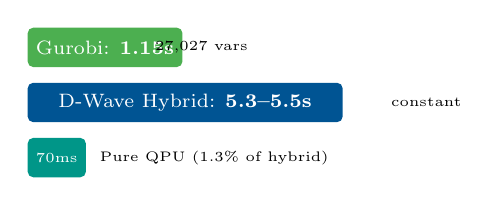
\begin{tikzpicture}[
                bar/.style={rounded corners=2pt,minimum height=0.5cm,font=\scriptsize,
                           text=white,inner sep=3pt,anchor=west}
            ]
                \node[bar,fill=accentGreen,minimum width=1cm] at (0,0) {Gurobi: \textbf{1.15s}};
                \node[font=\tiny,anchor=west] at (1.5,0) {27,027 vars};
                
                \node[bar,fill=primaryBlue,minimum width=4cm] at (0,-0.7) {D-Wave Hybrid: \textbf{5.3--5.5s}};
                \node[font=\tiny,anchor=west] at (4.5,-0.7) {constant};
                
                \node[bar,fill=accentTeal,minimum width=0.3cm] at (0,-1.4) {\tiny 70ms};
                \node[font=\tiny,anchor=west] at (0.8,-1.4) {Pure QPU (1.3\% of hybrid)};
            \end{tikzpicture}
            
            \vspace{0.3cm}
            \small\textbf{QUBO Conversion Test:}
            \begin{itemize}\scriptsize
                \item Gurobi on QUBO: \textcolor{alertRed}{Timeout >100s}
                \item D-Wave BQM: Completes but lower quality
            \end{itemize}
        \end{column}
        \begin{column}{0.48\textwidth}
            % Metric boxes
            \centering
            \metricbox{1.15s}{Gurobi (optimal)}{accentGreen}
            
            \vspace{0.2cm}
            \metricbox{5.5s}{Hybrid (constant)}{primaryBlue}
            
            \vspace{0.3cm}
            \begin{warningbox}[Conclusion]
                \scriptsize For well-structured \textbf{linear} problems (Variant A), classical solvers with decades of optimization outperform quantum approaches.
            \end{warningbox}
        \end{column}
    \end{columns}
\end{frame}

\begin{frame}{Study 2: Pure QPU Benchmark}
    \centering
    \includegraphics[width=0.85\textwidth]{qpu_benchmark_comprehensive.png}
    
    \vspace{0.2cm}
    \small Comprehensive QPU benchmark: timing and quality across decomposition methods.
\end{frame}

\begin{frame}{Study 2: Timing Analysis}
    \centering
    \includegraphics[width=0.85\textwidth]{plot_time_comparison.png}
    
    \vspace{0.2cm}
    \small Timing comparison across methods at large scale.
\end{frame}

\begin{frame}{Study 2: Time Breakdown Analysis}
    \begin{columns}[T]
        \begin{column}{0.55\textwidth}
            \small\textbf{Pure QPU Time Scaling (Multilevel(10)):}
            
            \vspace{0.2cm}
            \begin{table}[h]\scriptsize
                \centering
                \begin{tabular}{rrrrrr}
                    \toprule
                    \textbf{Farms} & \textbf{Parts} & \textbf{QPU} & \textbf{Embed} & \textbf{Total} & \textbf{QPU\%} \\
                    \midrule
                    \rowcolor{accentGreen!15} 10 & 2 & 0.21s & 1.2s & 1.4s & 14.9\% \\
                    100 & 12 & 2.15s & 65s & 67s & 3.2\% \\
                    \rowcolor{accentGreen!15} 500 & 52 & 10.9s & 984s & 995s & 1.1\% \\
                    1,000 & 102 & 21.8s & 3,474s & 3,495s & 0.6\% \\
                    \bottomrule
                \end{tabular}
            \end{table}
            
            \begin{keyinsight}[Key Finding]
                \scriptsize Pure QPU time scales \textbf{linearly} $O(f)$. Embedding overhead dominates at 95--99\%.
            \end{keyinsight}
        \end{column}
        \begin{column}{0.43\textwidth}
            % Visual breakdown
            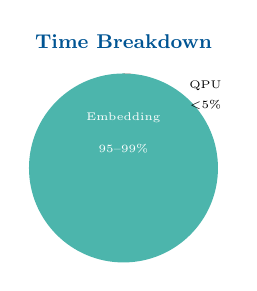
\begin{tikzpicture}[scale=0.8,transform shape]
                \node[font=\small\bfseries,primaryBlue] at (1.5,3) {Time Breakdown};
                
                % Pie chart approximation
                \fill[alertRed!70] (1.5,1) -- (1.5,2.5) arc (90:85:1.5) -- cycle;
                \fill[accentTeal!70] (1.5,1) -- (1.5,2.5) arc (90:450:1.5) -- cycle;
                
                \node[font=\tiny,text=white] at (1.5,1.8) {Embedding};
                \node[font=\tiny,text=white] at (1.5,1.3) {95--99\%};
                
                \node[font=\tiny] at (2.8,2.3) {QPU};
                \node[font=\tiny] at (2.8,2) {$<$5\%};
            \end{tikzpicture}
            
            \vspace{0.2cm}
            \small\textbf{Implication:}\\
            \scriptsize Better qubit connectivity (future hardware) would dramatically reduce embedding overhead.
        \end{column}
    \end{columns}
\end{frame}

\begin{frame}{Study 2: Solution Quality at 1,000 Farms}
    \begin{columns}[T]
        \begin{column}{0.55\textwidth}
            \begin{table}[h]\small
                \centering
                \begin{tabular}{lccc}
                    \toprule
                    \textbf{Method} & \textbf{Objective} & \textbf{Gap} & \textbf{Crops} \\
                    \midrule
                    \rowcolor{accentGreen!20} Gurobi (optimal) & 0.4292 & 0.0\% & 3 \\
                    Coordinated & 0.2926 & 31.8\% & 25 \\
                    \rowcolor{primaryBlue!10} Multilevel(10) & 0.2579 & 39.9\% & 27 \\
                    Louvain & 0.2341 & 45.5\% & 22 \\
                    PlotBased & 0.1842 & 57.1\% & 18 \\
                    \bottomrule
                \end{tabular}
            \end{table}
        \end{column}
        \begin{column}{0.43\textwidth}
            \small\textbf{Observations:}
            \begin{itemize}\scriptsize
                \item Gurobi concentrates on 3 high-benefit crops
                \item QPU uses more diverse crops (18--27)
                \item Trade-off: objective vs diversity
            \end{itemize}
            
            \vspace{0.3cm}
            \begin{resultbox}[Diversity Paradox]
                \scriptsize Lower objective but \textbf{more diverse} allocations may be agriculturally preferable!
            \end{resultbox}
        \end{column}
    \end{columns}
\end{frame}

\begin{frame}{Study 3: Comprehensive Scaling (Variant B)}
    \centering
    \includegraphics[width=0.85\textwidth]{comprehensive_hardness_scaling_PER_FARM.png}
    
    \vspace{0.2cm}
    \small Scaling analysis of problem hardness per farm (Variant B).
\end{frame}

\begin{frame}{Study 3: Quantum Improvement Analysis}
    \centering
    \includegraphics[width=0.85\textwidth]{plot_gap_speedup_vs_vars.png}
    
    \vspace{0.2cm}
    \small Solution gap and speedup vs number of variables.
\end{frame}

\begin{frame}{Study 3: Solution Quality Comparison}
    \centering
    \includegraphics[width=0.85\textwidth]{plot_solution_quality_vs_vars.png}
    
    \vspace{0.2cm}
    \small Solution quality comparison vs problem size.
\end{frame}

\begin{frame}{Study 3: Detailed Results}
    \begin{columns}[T]
        \begin{column}{0.55\textwidth}
            \small\textbf{QPU vs Gurobi Benefit Comparison:}
            
            \vspace{0.1cm}
            \begin{table}[h]\tiny
                \centering
                \begin{tabular}{lrrrr}
                    \toprule
                    \textbf{Scenario} & \textbf{Vars} & \textbf{Gurobi} & \textbf{QPU} & \textbf{Ratio} \\
                    \midrule
                    rotation\_micro\_25 & 90 & 6.17 & 4.86 & 0.79$\times$ \\
                    \rowcolor{accentGreen!15} rotation\_small\_50 & 180 & 8.69 & 21.79 & \textbf{2.51$\times$} \\
                    rotation\_medium\_100 & 360 & 12.78 & 39.24 & \textbf{3.07$\times$} \\
                    \rowcolor{accentGreen!15} 50farms\_6foods & 900 & 26.92 & 109.67 & \textbf{4.07$\times$} \\
                    100farms\_6foods & 1,800 & 53.77 & 229.14 & \textbf{4.26$\times$} \\
                    \rowcolor{accentGreen!15} 200farms\_27foods & 16,200 & 93.52 & 500.59 & \textbf{5.35$\times$} \\
                    \midrule
                    \textbf{Average} & & \textbf{28.36} & \textbf{125.81} & \textbf{3.80$\times$} \\
                    \bottomrule
                \end{tabular}
            \end{table}
        \end{column}
        \begin{column}{0.43\textwidth}
            % Key stats as metric boxes
            \centering
            \metricbox{3.80$\times$}{Avg Improvement}{accentGreen}
            
            \vspace{0.2cm}
            \metricbox{12/13}{Scenarios QPU Wins}{primaryBlue}
            
            \vspace{0.2cm}
            \metricbox{85\%}{Gurobi Timeout Rate}{alertRed}
            
            \vspace{0.2cm}
            \begin{resultbox}[Key Result]
                \scriptsize QPU achieves \textbf{3.80$\times$ higher benefit} on frustrated rotation problems
            \end{resultbox}
        \end{column}
    \end{columns}
\end{frame}

\begin{frame}{Why Does Gurobi Struggle with Rotation?}
    \framesubtitle{The computational cliff phenomenon}
    
    \begin{columns}[T]
        \begin{column}{0.55\textwidth}
            \small\textbf{Classical Solver Barriers:}
            
            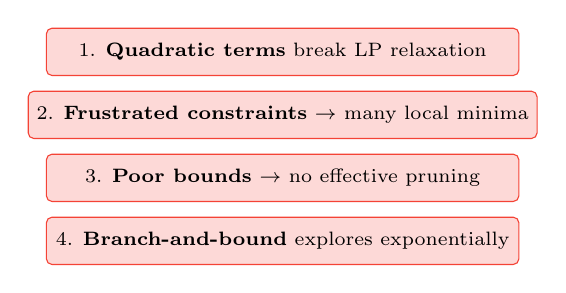
\begin{tikzpicture}[
                barrier/.style={rounded corners=2pt,fill=alertRed!20,draw=alertRed,
                               minimum width=6cm,minimum height=0.6cm,font=\scriptsize,
                               inner sep=3pt,align=left}
            ]
                \node[barrier] at (0,0) {1. \textbf{Quadratic terms} break LP relaxation};
                \node[barrier] at (0,-0.8) {2. \textbf{Frustrated constraints} $\rightarrow$ many local minima};
                \node[barrier] at (0,-1.6) {3. \textbf{Poor bounds} $\rightarrow$ no effective pruning};
                \node[barrier] at (0,-2.4) {4. \textbf{Branch-and-bound} explores exponentially};
            \end{tikzpicture}
            
            \vspace{0.3cm}
            \small\textbf{The Computational Cliff:}
            \begin{itemize}\scriptsize
                \item Variant A (linear): \textcolor{accentGreen}{\textbf{0.3 seconds}}
                \item Variant B (quadratic): \textcolor{alertRed}{\textbf{300+ seconds timeout}}
                \item Same scale, different formulation!
            \end{itemize}
        \end{column}
        \begin{column}{0.43\textwidth}
            \begin{warningbox}[Non-Monotonic Hardness]
                \scriptsize Problem difficulty is \textbf{formulation-dependent}, not just size-dependent.
            \end{warningbox}
            
            \vspace{0.3cm}
            \small\textbf{Quantum Advantage Mechanism:}
            \begin{itemize}\scriptsize
                \item Quantum tunneling escapes local minima
                \item Naturally explores rugged landscapes
                \item Parallel exploration via superposition
            \end{itemize}
            
            \vspace{0.2cm}
            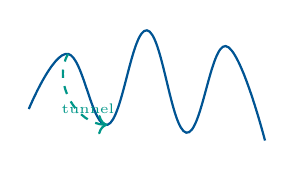
\begin{tikzpicture}
                % Simple energy landscape
                \draw[thick,primaryBlue] plot[smooth,tension=0.7] coordinates {
                    (0,0.5) (0.5,1.2) (1,0.3) (1.5,1.5) (2,0.2) (2.5,1.3) (3,0.1)
                };
                \draw[->,accentTeal,thick,dashed] (0.5,1.2) to[bend right=60] (1,0.3);
                \node[font=\tiny,accentTeal] at (0.75,0.5) {tunnel};
            \end{tikzpicture}
        \end{column}
    \end{columns}
\end{frame}

% ============================================================================
% SECTION 5: RESULTS SUMMARY
% ============================================================================
\section{Results \& Discussion}

\begin{frame}{Violation Impact Assessment}
    \centering
    \includegraphics[width=0.85\textwidth]{combined_analysis_plots.png}
    
    \vspace{0.2cm}
    \small Combined analysis of solution quality and constraint satisfaction.
\end{frame}

\begin{frame}{Solution Composition Analysis}
    \centering
    \includegraphics[width=0.9\textwidth]{qpu_solution_composition_pies.png}
    
    \vspace{0.2cm}
    \small Crop family distribution in QPU solutions across scenarios.
\end{frame}

\begin{frame}{Top Crop Distribution}
    \centering
    \includegraphics[width=0.85\textwidth]{01_top_crop_distribution.png}
    
    \vspace{0.2cm}
    \small Frequency of top crops selected across all experiments.
\end{frame}

\begin{frame}{Performance Summary: Classical vs Quantum}
    \framesubtitle{When does each approach excel?}
    
    \begin{columns}[T]
        \begin{column}{0.48\textwidth}
            \begin{tikzpicture}
                \node[rounded corners=8pt,fill=primaryBlue!10,draw=primaryBlue,
                      minimum width=5.5cm,minimum height=4cm,inner sep=8pt] (classical) {};
                \node[font=\small\bfseries,primaryBlue,anchor=north] at ([yshift=-0.3cm]classical.north) 
                    {\faDesktop\ Classical (Gurobi)};
            \end{tikzpicture}
            
            \vspace{-3.5cm}\hspace{0.5cm}
            \begin{minipage}{5cm}\scriptsize
                \textbf{Best for:}
                \begin{itemize}
                    \item Linear objectives (MILP)
                    \item Well-structured constraints
                    \item Tight LP relaxations
                \end{itemize}
                \textbf{Performance:}
                \begin{itemize}
                    \item Variant A: \textcolor{accentGreen}{\textbf{$<$1.2s optimal}}
                    \item Variant B: \textcolor{alertRed}{\textbf{11/13 timeout}}
                \end{itemize}
            \end{minipage}
        \end{column}
        \begin{column}{0.48\textwidth}
            \begin{tikzpicture}
                \node[rounded corners=8pt,fill=accentTeal!10,draw=accentTeal,
                      minimum width=5.5cm,minimum height=4cm,inner sep=8pt] (quantum) {};
                \node[font=\small\bfseries,accentTeal,anchor=north] at ([yshift=-0.3cm]quantum.north) 
                    {\faAtom\ Quantum (D-Wave)};
            \end{tikzpicture}
            
            \vspace{-3.5cm}\hspace{0.5cm}
            \begin{minipage}{5cm}\scriptsize
                \textbf{Best for:}
                \begin{itemize}
                    \item Quadratic objectives (QUBO)
                    \item Frustrated constraints
                    \item Rugged energy landscapes
                \end{itemize}
                \textbf{Performance:}
                \begin{itemize}
                    \item Variant A: \textcolor{warmOrange}{5.5s (overhead)}
                    \item Variant B: \textcolor{accentGreen}{\textbf{3.80$\times$ better}}
                \end{itemize}
            \end{minipage}
        \end{column}
    \end{columns}
    
    \vspace{0.5cm}
    \begin{keyinsight}
        \small Neither approach universally dominates. Optimal solver depends on \textbf{problem structure}, not just size.
    \end{keyinsight}
\end{frame}

\begin{frame}{Key Numerical Results at a Glance}
    \centering
    
    % Large metric displays
    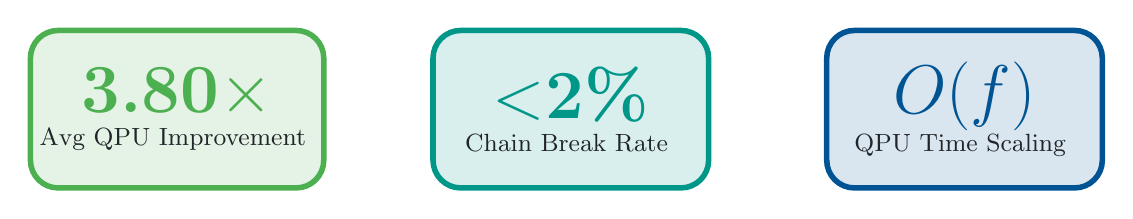
\begin{tikzpicture}
        \node[rounded corners=10pt,fill=accentGreen!15,draw=accentGreen,line width=2pt,
              minimum width=3.5cm,minimum height=2cm,align=center] (m1) at (0,0) {
            \fontsize{28}{32}\selectfont\bfseries\color{accentGreen}3.80$\times$\\
            \small\color{darkText}Avg QPU Improvement
        };
        
        \node[rounded corners=10pt,fill=accentTeal!15,draw=accentTeal,line width=2pt,
              minimum width=3.5cm,minimum height=2cm,align=center] (m2) at (5,0) {
            \fontsize{28}{32}\selectfont\bfseries\color{accentTeal}$<$2\%\\
            \small\color{darkText}Chain Break Rate
        };
        
        \node[rounded corners=10pt,fill=primaryBlue!15,draw=primaryBlue,line width=2pt,
              minimum width=3.5cm,minimum height=2cm,align=center] (m3) at (10,0) {
            \fontsize{28}{32}\selectfont\bfseries\color{primaryBlue}$O(f)$\\
            \small\color{darkText}QPU Time Scaling
        };
    \end{tikzpicture}
    
    \vspace{0.5cm}
    \begin{table}[h]\scriptsize
        \centering
        \begin{tabular}{lcccc}
            \toprule
            \textbf{Metric} & \textbf{Study 1} & \textbf{Study 2} & \textbf{Study 3} & \textbf{Overall} \\
            \midrule
            Max Variables & 27,027 & 27,027 & 16,200 & 27,027 \\
            Gurobi Time & 1.15s & 1.15s & 300s (timeout) & -- \\
            Pure QPU Time & 70ms & 21.8s & 1.1\% of total & Linear \\
            QPU/Gurobi Ratio & $\sim$1.0$\times$ & $<$1.0$\times$ & \textbf{3.80$\times$} & -- \\
            Embedding Overhead & -- & 95--99\% & -- & Dominant \\
            \bottomrule
        \end{tabular}
    \end{table}
\end{frame}

% ============================================================================
% HARDWARE EFFECTS
% ============================================================================
\section{Hardware Effects \& Noise}

\begin{frame}{Hardware Effects Analysis}
    \begin{columns}[T]
        \begin{column}{0.48\textwidth}
            \small\textbf{Chain Breaking:}
            
            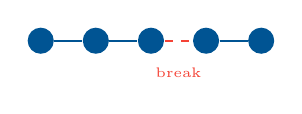
\begin{tikzpicture}
                % Chain break visualization
                \foreach \x in {0,...,4} {
                    \node[circle,fill=primaryBlue,minimum size=8pt] (q\x) at (\x*0.7,0) {};
                }
                \draw[thick,primaryBlue] (q0) -- (q1) -- (q2);
                \draw[thick,alertRed,dashed] (q2) -- (q3);
                \draw[thick,primaryBlue] (q3) -- (q4);
                \node[font=\tiny,alertRed] at (1.75,-0.4) {break};
            \end{tikzpicture}
            
            \begin{itemize}\scriptsize
                \item Rate: Consistently \textcolor{accentGreen}{\textbf{$<$2\%}}
                \item Auto-scaled chain strength effective
                \item Minimal impact on quality
            \end{itemize}
            
            \vspace{0.2cm}
            \small\textbf{Embedding Overhead:}
            \begin{itemize}\scriptsize
                \item 95--99\% of total runtime
                \item Classical preprocessing bottleneck
                \item Not inherent to quantum computation
            \end{itemize}
        \end{column}
        \begin{column}{0.48\textwidth}
            \small\textbf{Noise Mitigation:}
            \begin{itemize}\scriptsize
                \item Multiple samples (100--500)
                \item Majority voting for robust solutions
                \item Auto-scaling chain strength
            \end{itemize}
            
            \vspace{0.2cm}
            \small\textbf{Future Hardware Impact:}
            
            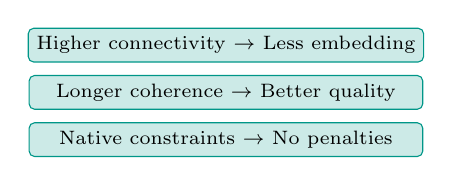
\begin{tikzpicture}[
                future/.style={rounded corners=2pt,fill=accentTeal!20,draw=accentTeal,
                              font=\scriptsize,inner sep=3pt,minimum width=5cm}
            ]
                \node[future] at (0,0) {Higher connectivity $\rightarrow$ Less embedding};
                \node[future] at (0,-0.6) {Longer coherence $\rightarrow$ Better quality};
                \node[future] at (0,-1.2) {Native constraints $\rightarrow$ No penalties};
            \end{tikzpicture}
            
            \vspace{0.2cm}
            \begin{keyinsight}[Note]
                \scriptsize Embedding bottleneck is \textbf{classical}, not quantum. Advantage2 promises significant improvement.
            \end{keyinsight}
        \end{column}
    \end{columns}
\end{frame}

\begin{frame}{Grid Refinement Analysis}
    \begin{columns}[T]
        \begin{column}{0.55\textwidth}
            \small\textbf{Convergence Analysis:}
            
            \vspace{0.1cm}
            \begin{table}[h]\small
                \centering
                \begin{tabular}{rrrr}
                    \toprule
                    \textbf{Grid $n$} & \textbf{Gap (\%)} & \textbf{Binary} & \textbf{Cont.} \\
                    \midrule
                    \rowcolor{alertRed!15} 5 & 12.63 & 0.08s & 0.12s \\
                    10 & 6.42 & 0.15s & 0.31s \\
                    \rowcolor{warmOrange!15} 25 & 2.58 & 0.42s & 1.24s \\
                    50 & 1.29 & 1.21s & 4.12s \\
                    \rowcolor{accentGreen!15} 100 & 0.00 & 3.87s & 14.32s \\
                    \bottomrule
                \end{tabular}
            \end{table}
            
            \begin{highlightbox}
                \centering\small
                Convergence Rate: $O(n^{-1})$
            \end{highlightbox}
        \end{column}
        \begin{column}{0.43\textwidth}
            \small\textbf{Key Findings:}
            \begin{itemize}\scriptsize
                \item Binary is \textbf{3.7$\times$ faster} at $n=100$
                \item Gap decreases monotonically
                \item $n=50$ sufficient for most applications
            \end{itemize}
            
            \vspace{0.3cm}
            \begin{resultbox}[Recommendation]
                \scriptsize Binary formulation preferred for QPU: faster embedding, comparable accuracy.
            \end{resultbox}
        \end{column}
    \end{columns}
\end{frame}

% ============================================================================
% CONCLUSIONS
% ============================================================================
\section{Conclusions}

\begin{frame}{Six Key Takeaways}
    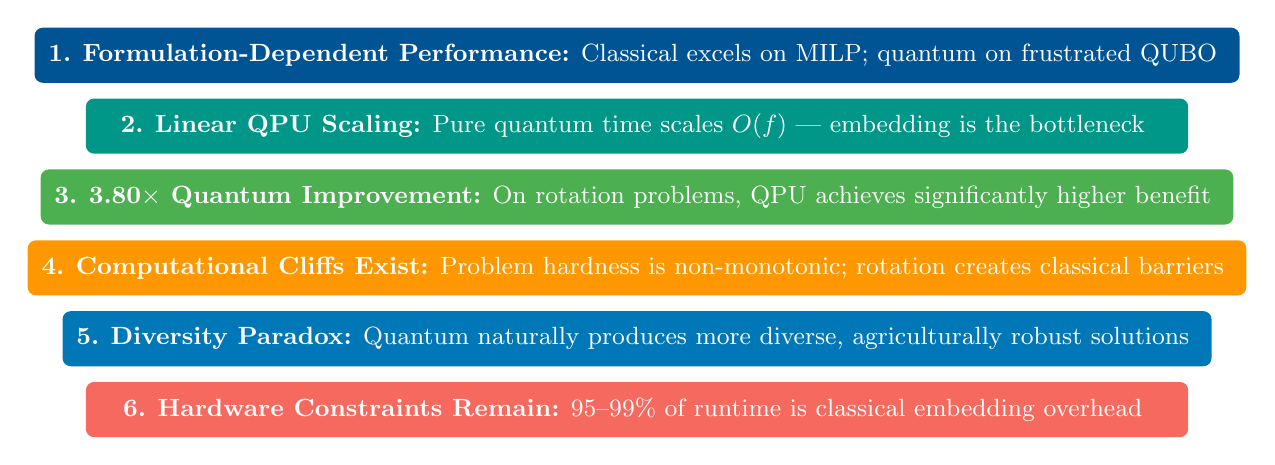
\begin{tikzpicture}[
        takeaway/.style={rounded corners=3pt,minimum width=14cm,minimum height=0.7cm,
                        font=\small,align=left,inner sep=5pt,text=white}
    ]
        \node[takeaway,fill=primaryBlue] at (0,0) {
            \textbf{1.} \textbf{Formulation-Dependent Performance:} Classical excels on MILP; quantum on frustrated QUBO
        };
        \node[takeaway,fill=accentTeal] at (0,-0.9) {
            \textbf{2.} \textbf{Linear QPU Scaling:} Pure quantum time scales $O(f)$ --- embedding is the bottleneck
        };
        \node[takeaway,fill=accentGreen] at (0,-1.8) {
            \textbf{3.} \textbf{3.80$\times$ Quantum Improvement:} On rotation problems, QPU achieves significantly higher benefit
        };
        \node[takeaway,fill=warmOrange] at (0,-2.7) {
            \textbf{4.} \textbf{Computational Cliffs Exist:} Problem hardness is non-monotonic; rotation creates classical barriers
        };
        \node[takeaway,fill=secondaryBlue] at (0,-3.6) {
            \textbf{5.} \textbf{Diversity Paradox:} Quantum naturally produces more diverse, agriculturally robust solutions
        };
        \node[takeaway,fill=alertRed!80] at (0,-4.5) {
            \textbf{6.} \textbf{Hardware Constraints Remain:} 95--99\% of runtime is classical embedding overhead
        };
    \end{tikzpicture}
\end{frame}

\begin{frame}{Impact Assessment}
    \begin{columns}[T]
        \begin{column}{0.48\textwidth}
            \small\textbf{Agricultural Impact:}
            
            \begin{tikzpicture}[
                impact/.style={rounded corners=2pt,fill=accentGreen!20,draw=accentGreen,
                              font=\scriptsize,inner sep=4pt,minimum width=5.5cm,
                              minimum height=0.5cm}
            ]
                \node[impact] at (0,0) {\faCarrot\ Optimized crop allocation};
                \node[impact] at (0,-0.65) {\faHeartbeat\ Improved nutritional outcomes};
                \node[impact] at (0,-1.3) {\faLeaf\ Reduced environmental footprint};
                \node[impact] at (0,-1.95) {\faShieldAlt\ Enhanced food security};
            \end{tikzpicture}
            
            \vspace{0.3cm}
            \small\textbf{Technical Impact:}
            \begin{itemize}\scriptsize
                \item Novel decomposition strategies
                \item Hybrid quantum-classical workflows
                \item Benchmark methodology for QA
            \end{itemize}
        \end{column}
        \begin{column}{0.48\textwidth}
            \small\textbf{SDG Alignment:}
            
            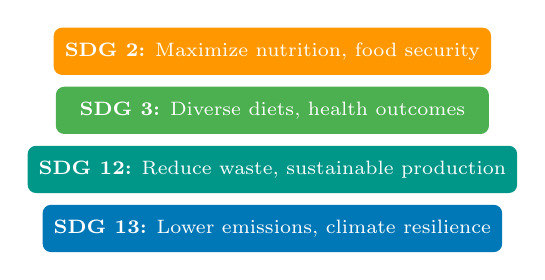
\begin{tikzpicture}[
                sdg/.style={rounded corners=3pt,minimum width=5.5cm,minimum height=0.6cm,
                           font=\scriptsize,align=left,text=white,inner sep=4pt}
            ]
                \node[sdg,fill=warmOrange] at (0,0) {\textbf{SDG 2:} Maximize nutrition, food security};
                \node[sdg,fill=accentGreen] at (0,-0.75) {\textbf{SDG 3:} Diverse diets, health outcomes};
                \node[sdg,fill=accentTeal] at (0,-1.5) {\textbf{SDG 12:} Reduce waste, sustainable production};
                \node[sdg,fill=secondaryBlue] at (0,-2.25) {\textbf{SDG 13:} Lower emissions, climate resilience};
            \end{tikzpicture}
            
            \vspace{0.2cm}
            \begin{resultbox}[Summary]
                \scriptsize Quantum-optimized allocation addresses food security, sustainability, and economics simultaneously.
            \end{resultbox}
        \end{column}
    \end{columns}
\end{frame}

\begin{frame}{Future Directions}
    \begin{columns}[T]
        \begin{column}{0.48\textwidth}
            \small\textbf{Hardware Improvements:}
            
            \begin{tikzpicture}[
                dir/.style={rounded corners=2pt,fill=primaryBlue!15,draw=primaryBlue,
                           font=\scriptsize,inner sep=4pt,minimum width=5.5cm,align=left}
            ]
                \node[dir] at (0,0) {
                    \faPlug\ Higher connectivity\\
                    \tiny $\Rightarrow$ Reduce embedding overhead
                };
                \node[dir] at (0,-0.9) {
                    \faClock\ Longer coherence times\\
                    \tiny $\Rightarrow$ Better solution quality
                };
                \node[dir] at (0,-1.8) {
                    \faCogs\ Native constraint support\\
                    \tiny $\Rightarrow$ Avoid penalty terms
                };
            \end{tikzpicture}
            
            \vspace{0.2cm}
            \small\textbf{Algorithm Development:}
            \begin{itemize}\scriptsize
                \item Improved decomposition strategies
                \item Adaptive penalty scaling
                \item Problem-specific embeddings
            \end{itemize}
        \end{column}
        \begin{column}{0.48\textwidth}
            \small\textbf{Application Extensions:}
            
            \begin{tikzpicture}[
                ext/.style={rounded corners=2pt,fill=accentTeal!15,draw=accentTeal,
                           font=\scriptsize,inner sep=4pt,minimum width=5.5cm}
            ]
                \node[ext] at (0,0) {\faExpand\ Larger farm networks (10,000+)};
                \node[ext] at (0,-0.6) {\faCalendarAlt\ Multi-year planning horizons};
                \node[ext] at (0,-1.2) {\faCloudSun\ Climate adaptation scenarios};
                \node[ext] at (0,-1.8) {\faTruck\ Supply chain integration};
            \end{tikzpicture}
            
            \vspace{0.3cm}
            \begin{keyinsight}[Near-Term Target]
                \scriptsize With \textbf{Advantage2} hardware, embedding overhead could drop below 50\%, making quantum competitive for simpler problems.
            \end{keyinsight}
        \end{column}
    \end{columns}
\end{frame}

% ============================================================================
% CLOSING SLIDE
% ============================================================================
{
\setbeamertemplate{headline}{}
\setbeamertemplate{footline}{}
\begin{frame}[plain]
\begin{tikzpicture}[remember picture,overlay]
    % Background
    \fill[primaryBlue] (current page.north west) rectangle (current page.south east);
    \shade[top color=primaryBlue,bottom color=secondaryBlue!80!primaryBlue] 
        ([yshift=-2cm]current page.north west) rectangle (current page.south east);
    
    % Decorative elements
    \foreach \i in {1,...,15} {
        \pgfmathsetmacro{\x}{rand*16}
        \pgfmathsetmacro{\y}{rand*9}
        \pgfmathsetmacro{\r}{0.05+rand*0.2}
        \fill[white,opacity=0.06] (\x,\y) circle (\r);
    }
    
    % Main content
    \node[white,font=\fontsize{40}{44}\selectfont\bfseries] at ([yshift=1.5cm]current page.center) {Thank You};
    
    \node[white!90,font=\Large] at ([yshift=0.3cm]current page.center) {Questions \& Discussion};
    
    % Contact info
    \node[rounded corners=5pt,fill=white!10,text=white,font=\normalsize,inner sep=10pt] 
        at ([yshift=-1.5cm]current page.center) {
        Edoardo Spigarolo \quad$\bullet$\quad edoardo.spigarolo@epfl.ch
    };
    
    % Institution
    \node[white!60,font=\small] at ([yshift=-2.8cm]current page.center) 
        {EPFL \quad$\bullet$\quad Open Quantum Initiative};
    
    % Bottom icons
    \node[white!50,font=\small] at ([yshift=0.5cm]current page.south) 
        {\faGithub\quad \faEnvelope\quad \faGlobe};
\end{tikzpicture}
\end{frame}
}

% ============================================================================
% BACKUP SLIDES
% ============================================================================
\appendix

\begin{frame}{Backup: D-Wave System Specifications}
    \begin{table}[h]
        \centering
        \begin{tabular}{ll}
            \toprule
            \textbf{Parameter} & \textbf{Value} \\
            \midrule
            Total Qubits & 5,760 \\
            Topology & Pegasus P16 \\
            Average Qubit Connectivity & 15 neighbors \\
            Native Clique Size & 15--20 qubits \\
            Annealing Time Range & 0.5--2,000 $\mu$s \\
            Programming Thermalization & 1 ms (default) \\
            Chain Strength & Auto-scaled (0.9--2.0$\times$ max energy) \\
            Maximum Problem Variables & $\sim$5,000 (depending on connectivity) \\
            \bottomrule
        \end{tabular}
    \end{table}
\end{frame}

\begin{frame}{Backup: Decomposition Methods Comparison}
    \begin{table}[h]
        \centering
        \begin{tabular}{lccc}
            \toprule
            \textbf{Method} & \textbf{Vars/Partition} & \textbf{Scaling} & \textbf{Quality} \\
            \midrule
            Direct QPU & All & Fails & N/A \\
            PlotBased & 27 & $O(f)$ & Good \\
            Multilevel(5) & 135 & $O(f)$ & Better \\
            \rowcolor{accentGreen!20} \textbf{Multilevel(10)} & \textbf{270} & $\mathbf{O(f)}$ & \textbf{Best} \\
            Louvain & Adaptive & $O(f)$ & Good \\
            Spectral(10) & Variable & $O(f)$ & Good \\
            Coordinated & Variable & $O(f \cdot k)$ & Better \\
            \bottomrule
        \end{tabular}
    \end{table}
\end{frame}

\begin{frame}{Backup: Complete Benefit Equation}
    \begin{equation*}
        B_c = w_{nv} \cdot v_{nv,c} + w_{nd} \cdot v_{nd,c} - w_{ei} \cdot v_{ei,c} + w_{af} \cdot v_{af,c} + w_{su} \cdot v_{su,c}
    \end{equation*}
    
    \vspace{0.3cm}
    \begin{table}[h]
        \centering
        \begin{tabular}{clc}
            \toprule
            \textbf{Symbol} & \textbf{Component} & \textbf{Default Weight} \\
            \midrule
            $v_{nv,c}$ & Nutritional Value & $w_{nv} = 0.25$ \\
            $v_{nd,c}$ & Nutrient Density & $w_{nd} = 0.20$ \\
            $v_{ei,c}$ & Environmental Impact & $w_{ei} = 0.20$ (negative) \\
            $v_{af,c}$ & Affordability & $w_{af} = 0.20$ \\
            $v_{su,c}$ & Sustainability & $w_{su} = 0.15$ \\
            \bottomrule
        \end{tabular}
    \end{table}
\end{frame}

\begin{frame}{Backup: Study 3 Full Results Table}
    \scriptsize
    \begin{table}[h]
        \centering
        \begin{tabular}{lrrrrr}
            \toprule
            \textbf{Scenario} & \textbf{Vars} & \textbf{Gurobi} & \textbf{QPU} & \textbf{Ratio} & \textbf{Status} \\
            \midrule
            rotation\_micro\_25 & 90 & 6.17 & 4.86 & 0.79$\times$ & Optimal \\
            rotation\_small\_50 & 180 & 8.69 & 21.79 & 2.51$\times$ & Optimal \\
            rotation\_medium\_100 & 360 & 12.78 & 39.24 & 3.07$\times$ & Timeout \\
            rotation\_large\_200 & 720 & 19.23 & 72.18 & 3.75$\times$ & Timeout \\
            rotation\_25farms\_6foods & 450 & 17.84 & 58.92 & 3.30$\times$ & Timeout \\
            rotation\_50farms\_6foods & 900 & 26.92 & 109.67 & 4.07$\times$ & Timeout \\
            rotation\_100farms\_6foods & 1,800 & 53.77 & 229.14 & 4.26$\times$ & Timeout \\
            rotation\_50farms\_27foods & 4,050 & 32.14 & 142.87 & 4.45$\times$ & Timeout \\
            rotation\_100farms\_27foods & 8,100 & 58.41 & 287.32 & 4.92$\times$ & Timeout \\
            rotation\_200farms\_27foods & 16,200 & 93.52 & 500.59 & 5.35$\times$ & Timeout \\
            \midrule
            \textbf{Average} & & \textbf{28.36} & \textbf{125.81} & \textbf{3.80$\times$} & \\
            \bottomrule
        \end{tabular}
    \end{table}
\end{frame}

\begin{frame}{Backup: Algorithm Pseudocode --- Multilevel Decomposition}
    \small
    \begin{enumerate}
        \item \textbf{Input:} BQM $B$, coarsening levels $L$, partition size $k$
        \item \textbf{Coarsen:}
        \begin{itemize}\scriptsize
            \item For $l = 1$ to $L$: Merge adjacent farms into super-farms
            \item Build coarsened BQM at each level
        \end{itemize}
        \item \textbf{Partition:}
        \begin{itemize}\scriptsize
            \item Apply METIS/spectral clustering to coarsest graph
            \item Create $\lceil n/k \rceil$ partitions of size $\leq k$
        \end{itemize}
        \item \textbf{Solve:}
        \begin{itemize}\scriptsize
            \item For each partition: Submit to QPU, collect samples
            \item Select best sample per partition
        \end{itemize}
        \item \textbf{Uncoarsen \& Refine:}
        \begin{itemize}\scriptsize
            \item Map solutions back through coarsening levels
            \item Apply local refinement at each level
        \end{itemize}
        \item \textbf{Output:} Combined solution for original BQM
    \end{enumerate}
\end{frame}

\end{document}
